\documentclass[8pt]{beamer}

\usetheme{Copenhagen}
\usecolortheme{beaver}
\usepackage[small,center]{caption}
\usepackage{times}
\usefonttheme{structurebold}
\usepackage[english]{babel}
\usepackage{pgf,pgfarrows,pgfnodes,pgfautomata,pgfheaps}
\usepackage{amsmath,amssymb}
\usepackage{amsxtra}

\usepackage{caption}
\usepackage{tikz}
\usetikzlibrary{shapes.misc}

\newcommand{\leftd}[1]{{\color{red} \bar{#1}}}
\newcommand{\interface}[2]{{\color{blue}{#1}_I(#2)}}
\newcommand{\leftdd}[2]{{\color{red} \bar{#1}(\bar{#2})}}
\newcommand{\leftFourier}[1]{{\color{red} \hat{#1}}}
\newcommand{\leftFourierTwo}[2]{{\color{red} \hat{#1}(\hat{#2})}}
\newcommand{\half}{\dfrac{1}{2}}
\newcommand{\divergence}{\mathrm{div}}

\newcommand{\I}{I}

\newcommand*{\vcenterimage}[1]{\vcenter{\hbox{\includegraphics[width=2in]{#1}}}}
\newcommand*{\vcenterarrow}{\vcenter{\hbox{$\Longrightarrow$}}}


\definecolor{RPIred}{rgb}{ 0.87,0.12, 0.20}
\definecolor{ballblue}{rgb}{0.13, 0.67, 0.8}
\definecolor{lightgray}{rgb}{0.83, 0.83, 0.83}
\setbeamercolor{block title}{bg=lightgray,fg=RPIred}
\setbeamercolor{block body}{bg=white,fg=black}
\setbeamercovered{dynamic}
\setbeamercolor*{item}{fg=RPIred}

\captionsetup[subfigure]{labelformat=empty}
\captionsetup[figure]{labelformat=empty}
\setbeamertemplate{navigation symbols}{}
\setbeamertemplate{footline}[frame number]
\begin{document}

% tikz stuff
\tikzset{cross/.style={cross out, draw=black, minimum size=2*(#1-\pgflinewidth),
inner sep=0pt, outer sep=0pt},
%default radius will be 1pt.
cross/.default={2.5pt}}



\frame{
\title{\Large Improving Boundary Derivative Accuracy with \(p\)-Refinement}

\author{{\Large David Wells \\\vspace{0.1in} Rensselaer Polytechnic Institute}\\
\vspace{0.2in} {In collaboration with:\\{}J. W. Banks, F. Li}}

\date{July 13, 2017\\{} SIAM Annual Meeting}

\begin{figure}[h]
\centering
\includegraphics[width=1.5in]{RPI_letterhead.pdf}
 \end{figure}%

\vspace{-0.2in}
\titlepage
}

\begin{frame}
    \frametitle{Outline}
    \begin{itemize}
    \item[$\blacksquare$] Goals                                               \\
    \item[$\blacksquare$] A Little on Superconvergence                        \\
    \item[$\blacksquare$] \(p\)-refinement results in 1D                      \\
    \item[$\blacksquare$] Extensions to 2D                                    \\
    \item[$\blacksquare$] Summary                                             \\
    \end{itemize}
\end{frame}

\section{Goals}
    \begin{frame}
        \frametitle{Goals}
        \begin{itemize}
            \item Efficient numerical methods for elliptic PDEs
            \item Increased accuracy in (normal) boundary derivatives
            \item No postprocessing
            \item Order \(n + 1\) data should lead to order \(n + 1\) derivatives
        \end{itemize}
    \end{frame}

    \begin{frame}
        \frametitle{Goals}
        \begin{center}
            (mostly) bilinear elements and order \(2\) accurate (normal)
            second derivatives (at isolated points)
        \end{center}
    \end{frame}

\section{Superconvergence}
\begin{frame}
    \frametitle{Assumptions}
    \begin{itemize}
        \item Linear, constant coefficient elliptic PDEs, Dirichlet (or
              periodic) boundary conditions
              \pause
        \item \emph{Lots} of regularity
              \pause
        \item Uniform grid (constant \(\Delta x\), \(\Delta y\)) of tensor
              product elements (no triangles)
              \pause
        \item Continuous finite element spaces
              \begin{itemize}
                  \item in 1D, degree \(n\) on interior elements, degree \(n +
                        p\) on nonperiodic edge elements
                  \item in 2D, bilinear on interior elements, degree \(1 \otimes
                        1 + p\) on nonperiodic edge elements
              \end{itemize}
              \pause
        \item Optimal \(L^\infty\) estimates in 1D
              \begin{equation*}
                  \left\|\dfrac{d^m}{dx^m}(u - u^h)\right\|_{L^\infty}
                  \leq C \left\|\dfrac{d^{m + 1}}{dx^{m + 1}} u\right\|_{L^\infty}
                  \Delta x^{n + 1- m}
              \end{equation*}
    \end{itemize}
\end{frame}

\begin{frame}
    \frametitle{What's the plan?}
    \begin{itemize}
        \item Static \(p\)-refinement: some cells have higher degree polynomial bases
        \item Global \(h\)-refinement: no mesh adaptivity (yet)
        \item Not really an \(hp\)-element method, but similar
    \end{itemize}
\end{frame}

\begin{frame}
    \frametitle{What's the plan?}
    \begin{center}
        Picking the right type of \(p\)-refinement improves the boundary
        derivative convergence rates.
    \end{center}
\end{frame}

\begin{frame}
    \frametitle{Superconvergence in 1D}
    \emph{Classic result}: continuous FE approximation of \(-u_{xx} = f\) with
    \(V^h =\) piecewise polynomials of degree \(n\) has \emph{zero error} at the
    knots (cell faces).                                                       \\

    \pause

    \emph{proof:} (Arnold et al, 1972) Consider a knot \(i \Delta x\):
    \begin{align*}
        |u^h(i \Delta x) - u(i \Delta x)|
        &= |a(G_{i\Delta x}, u^h - u)|                                        \\
        &= |a(G_{i\Delta x} - v^h, u^h - u)|                                  \\
        &\leq C \|G_{i\Delta x} - v^h\|_{H^1} \|u^h - u\|_{H^1}
    \end{align*}
    \pause
    \begin{itemize}
        \item \(G_{i\Delta x}\) is the Green's function centered at \(i \Delta
              x\)
        \item \(G_{i \Delta x}\) is piecewise linear
              \(\Rightarrow G_{i\Delta x} \in V^h\)
        \item Pick \(G_{i\Delta x} = v^h\): no knot error!
    \end{itemize}
\end{frame}

\begin{frame}
    \frametitle{Superconvergence in 1D}
    Same idea for \(-u_{xx} + b u_x + c u = f\):
    \pause
    \begin{align*}
        |u^h(i \Delta x) - u(i \Delta x)|
        &= |a(G_{i\Delta x}, u^h - u)|                                        \\
        &= |a(G_{i\Delta x} - v^h, u^h - u)|                                  \\
        &\leq C_1 \|G_{i\Delta x} - v^h\|_{H^1} \|u^h - u\|_{H^1}             \\
        &\leq C_2 \Delta x^{2 k}.
    \end{align*}
\end{frame}

\begin{frame}
    \frametitle{Superconvergence in 1D}
    Useful special case for CDR if the last cell consists of piecewise
    polynomials of degree \(n + p\), \(p \geq 1\), then
    \begin{equation*}
        |u(1 - \Delta x) - u^h(1 - \Delta x)| \leq C \Delta x^{2 n + 1}
    \end{equation*}
    \pause
    \emph{Proof}:
    \begin{itemize}
        \item Same work as before: knot error is bounded by global error times
              Green's function (interpolation) error
        \item To the left of \(1 - \Delta x\): derivatives of the Green's
              function scale like \(O(\Delta x) \Rightarrow\) we gain an
              approximation order
        \item To the right of \(1 - \Delta x\): \(p \geq 1 \Rightarrow\) we gain
              (at least) one approximation order
    \end{itemize}
\end{frame}

\section{\(p\)-refinement in 1D}
\begin{frame}
    \frametitle{Improving boundary derivative convergence in \(1D\)}
    Our first step towards the goal: improving boundary derivative approximation
    orders for
    \begin{equation*}
        -u_{xx} = f
    \end{equation*}
    \pause
    \begin{equation*}
        \left|\dfrac{d^m}{dx^m}(u - u^h)(1)\right|
        \leq C \Delta x^{n + p + 1 - m}
    \end{equation*}
    \pause
    \begin{itemize}
        \item FE scheme on the boundary cell, \(y^h\):
              \begin{itemize}
                  \item \(y^h(1 - \Delta x) = u^h(1 - \Delta x) = u(1 - \Delta x)\)
                  \item \(y^h(1) = u^h(1) = u(1)\)
              \end{itemize}
              \pause
        \item No knot errors
        \item Estimates on last cell \emph{don't rely on the rest of the
              domain}
        \item Equivalent, discretely, to just doing plain \(p\)-refinement on
              the last cell
    \end{itemize}
\end{frame}

\begin{frame}
    \frametitle{Improving boundary derivative convergence in 1D}
    For
    \begin{equation*}
        -u_{xx} + b u_x + c u = f
    \end{equation*}
    \pause
    \begin{equation*}
        \left|\dfrac{d^m}{dx^m}(u - u^h)(1)\right|
        \leq C_1 \Delta x^{n + p + 1 - m}
        + C_2 \Delta x^{2 n - 1}
    \end{equation*}
    \pause
    \begin{itemize}
        \item Same as the Laplace equation (\(C_1\)), but with a nonzero coupling error
              (saved by better knot estimate, \(C_2 \Delta x^{2 n - 1}\))
    \end{itemize}
    \pause
    \begin{center}
        \(n = 1, p = 2 \Rightarrow\) a second order accurate second derivative
        on the boundary.
    \end{center}
\end{frame}

\begin{frame}
    \frametitle{Numerical Results}
    Domain of \([0, 1]\), with manufactured solution
    \begin{equation*}
        u = \sin(10 x)
    \end{equation*}
    \begin{itemize}
        \item Use \texttt{deal.II}'s \(hp\)-finite element support
        \item Bulk order \(2\), boundary orders \(2\), \(3\), and \(4\)
        \item CDR equation
        \item Solve with GMRES
    \end{itemize}
\end{frame}

\begin{frame}
    \frametitle{Numerical Results}
    \begin{figure}
        \centering
        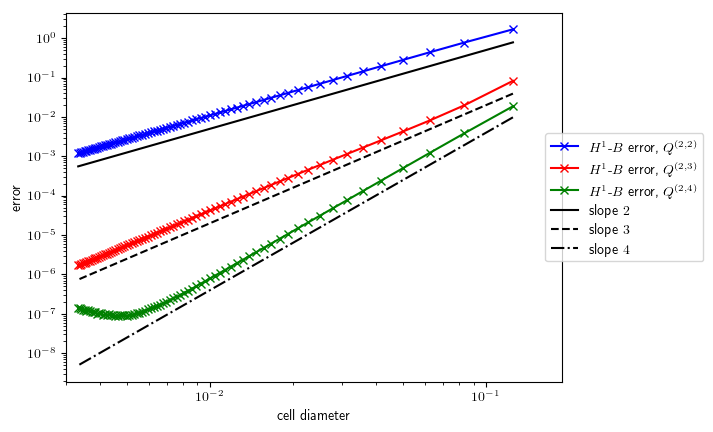
\includegraphics[width=4in]{Pictures/oned-cdr-2-h1-errors.png}

        \caption{Convergence rates for the \(p\)-refinement scheme of the
        first derivative on the boundary. We hit roundoff error near the end.}
    \end{figure}
\end{frame}

\begin{frame}
    \frametitle{Numerical Results}
    \begin{figure}
        \centering
        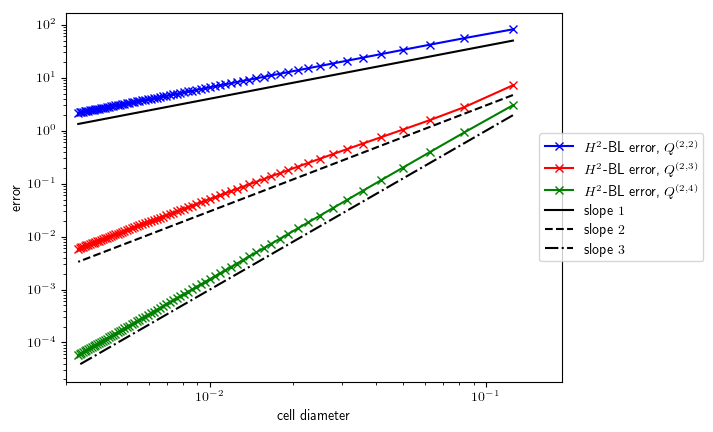
\includegraphics[width=4in]{Pictures/oned-cdr-2-h2-errors.png}

        \caption{Convergence rates for the \(p\)-refinement scheme of the second
        derivative on the boundary.}
    \end{figure}
\end{frame}

\section{\(p\)-refinement in 2D}
\begin{frame}
    \frametitle{Extensions to 2D}
    With periodic boundary conditions in \(x\) and Dirichlet boundary conditions
    in \(y\), \(\sqrt{-1} = I\):
    \begin{equation*}
        -\Delta u + \vec{b}\cdot\nabla u + c u = f
        \Rightarrow
        -\hat{u}_{yy} + b_2 \hat{u}_y + (k^2 + I k b_1 + c) \hat{u} = \hat{f}_k
    \end{equation*}
    If we can handle the Fourier transform somehow then we are set.
\end{frame}

\begin{frame}
    \frametitle{Extensions to 2D}
    \begin{itemize}
        \item Discretize in \(x\) and consider a semidiscretization in \(y\)
        \item Linear elements in \(x \Rightarrow\) centered differences in \(x\)
        \item The solution in \(x\) is a superposition of grid eigenfunctions
              \(\exp(I k x_i) \Rightarrow\) calculate errors for each \(k\) and
              sum them up via inverse discrete Fourier transform
    \end{itemize}
    \pause
    \vspace{0.25in}
    \begin{equation*}
        -Y_k''(y)
        + b_2 Y_k'(y)
        +
        \left(
        \dfrac{4 \sin^2(k \Delta x/2)}{\Delta x^2}
        + \dfrac{b_1 \I \sin(k \Delta x)}{\Delta x}
        + \dfrac{4 + 2 \cos(k \Delta x)}{6} c
        \right) Y_k(y)
        = F_k(y).
    \end{equation*}
\end{frame}

\begin{frame}
    \frametitle{Extensions to 2D}
    \begin{equation*}
        \left|
        \dfrac{d^m}{dx^m}
        \left(u(x, y) - u^h(x, y) \right)
        \bigg|_{(\delta_i, \delta_{N^*})}
        \right|
        \leq
        C_1 \Delta x^{2}
        +
        C_2 \Delta y^{2 + p - m}
    \end{equation*}
    where \(N^* = 0\) or \(N^* = N\).

    \emph{proof outline:}
    \begin{itemize}
        \item \(x\)-discretization is \(O(\Delta x^2)\) from the Fourier
              solution; higher-frequency modes have a small contribution
              (regularity assumption)
        \item Derivatives of the Green's function scale like \(O(k^{m - 1})\):
              controlled by the decay of the Fourier coefficients (regularity
              assumption)
        \item Sums in the inverse Fourier transform converge with no loss in
              approximation order
    \end{itemize}

    \emph{Important:} this only proves convergence at \emph{knots}.
\end{frame}

\begin{frame}
    \frametitle{Elimination of nonnormal \(p\)-refinement}
    \begin{figure}
        \centering

        \begin{tikzpicture}[scale=1.5]
    %% leftmost pair
    % cubic square
    \draw[-, thick] (-1.0, 0.0) -- (-1.0, 1.0);
    \draw[-, thick] (0.0, 0.0) -- (0.0, 1.0);
    \draw[-, thick] (-1.0, 0.0) -- (0.0, 0.0);
    \draw[-, thick] (-1.0, 1.0) -- (0.0, 1.0);

    % linear square
    \draw[-, thick] (-1.0, -1.0) -- (-1.0, 0.0);
    \draw[-, thick] (0.0, -1.0) -- (0.0, 0.0);
    \draw[-, thick] (-1.0, -1.0) -- (0.0, -1.0);
    \draw[-, thick] (-1.0, 0.0) -- (0.0, 0.0);

    % cubic support points
    \foreach \x in {0,...,4}
    \foreach \y in {0,...,4}
        \draw (0.25*\x - 1.0, 0.25*\y) node[cross] {};

    % linear support points
    \foreach \x in {0,...,1}
    \foreach \y in {0,...,1}
        \draw (\x - 1.0, \y - 1.0) circle (2pt);

    %% second pair
    % cubic square
    \draw[-, thick] (0.0, 0.0) -- (0.0, 1.0);
    \draw[-, thick] (1.0, 0.0) -- (1.0, 1.0);
    \draw[-, thick] (0.0, 0.0) -- (1.0, 0.0);
    \draw[-, thick] (0.0, 1.0) -- (1.0, 1.0);

    % linear square
    \draw[-, thick] (0.0, -1.0) -- (0.0, 0.0);
    \draw[-, thick] (1.0, -1.0) -- (1.0, 0.0);
    \draw[-, thick] (0.0, -1.0) -- (1.0, -1.0);
    \draw[-, thick] (0.0, 0.0) -- (1.0, 0.0);

    % cubic support points
    \foreach \x in {0,...,4}
    \foreach \y in {0,...,4}
        \draw (0.25*\x, 0.25*\y) node[cross] {};

    % linear support points
    \foreach \x in {0,...,1}
    \foreach \y in {0,...,1}
        \draw (\x, \y - 1.0) circle (2pt);

    \draw[->, thick] (1.5, 0.0) -- (2.5, 0.0);

    % cubic square
    \draw[-, thick] (3.0, 0.0) -- (3.0, 1.0);
    \draw[-, thick] (4.0, 0.0) -- (4.0, 1.0);
    \draw[-, thick] (3.0, 0.0) -- (4.0, 0.0);
    \draw[-, thick] (3.0, 1.0) -- (4.0, 1.0);

    % linear square
    \draw[-, thick] (3.0, -1.0) -- (3.0, 0.0);
    \draw[-, thick] (4.0, -1.0) -- (4.0, 0.0);
    \draw[-, thick] (3.0, -1.0) -- (4.0, -1.0);
    \draw[-, thick] (3.0, 0.0)  -- (4.0, 0.0);

    % cubic support points
    \foreach \x in {0,...,1}
    \foreach \y in {0,...,4}
        \draw (3.0 + \x, 0.25*\y) node[cross] {};

    % linear support points
    \foreach \x in {0,...,1}
    \foreach \y in {0,...,1}
        \draw (3.0 + \x, \y - 1.0) circle (2pt);

    %% rightmost pair
    % cubic square
    \draw[-, thick] (4.0, 0.0) -- (4.0, 1.0);
    \draw[-, thick] (5.0, 0.0) -- (5.0, 1.0);
    \draw[-, thick] (4.0, 0.0) -- (5.0, 0.0);
    \draw[-, thick] (4.0, 1.0) -- (5.0, 1.0);

    % linear square
    \draw[-, thick] (4.0, -1.0) -- (4.0, 0.0);
    \draw[-, thick] (5.0, -1.0) -- (5.0, 0.0);
    \draw[-, thick] (4.0, -1.0) -- (5.0, -1.0);
    \draw[-, thick] (4.0, 0.0)  -- (5.0, 0.0);

    % cubic support points
    \foreach \x in {0,...,1}
    \foreach \y in {0,...,4}
        \draw (4.0 + \x, 0.25*\y) node[cross] {};

    % linear support points
    \foreach \x in {0,...,1}
    \foreach \y in {0,...,1}
        \draw (4.0 + \x, \y - 1.0) circle (2pt);
\end{tikzpicture}

        \caption{Depiction of normal \(p\)-refinement scheme, with elimination
        of extra DoFs. Linear DoFs are circles, quartic are crosses.}
    \end{figure}
\end{frame}

\begin{frame}
    \frametitle{Numerical Results}
    \begin{figure}
        \centering
        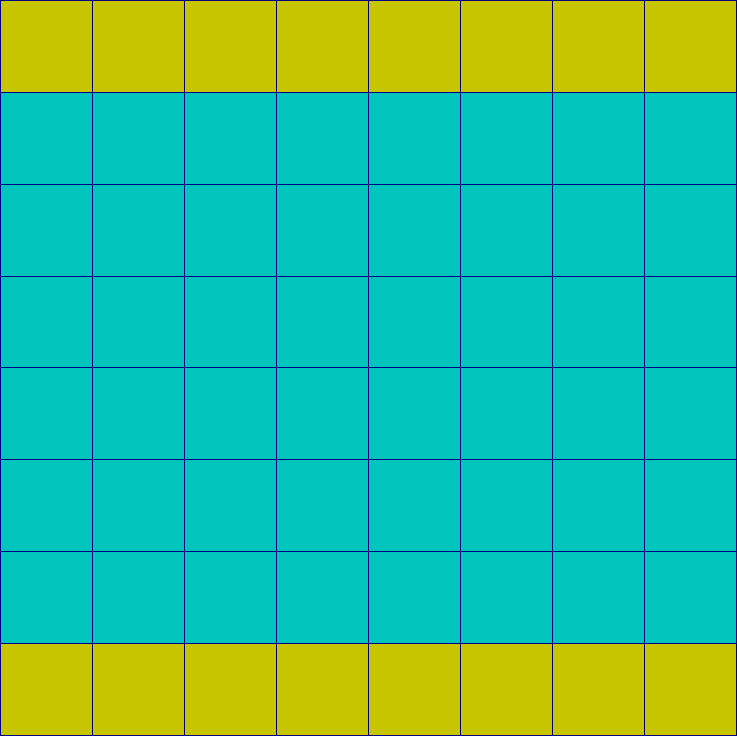
\includegraphics[width=2.5in]{Pictures/square-periodic-grid.png}

        \caption{Depiction of the square grid with bulk cells in cyan and
        \(p\)-refined cells in yellow.}
    \end{figure}
\end{frame}

\begin{frame}
    \frametitle{Numerical Results}
    \begin{figure}
        \centering
        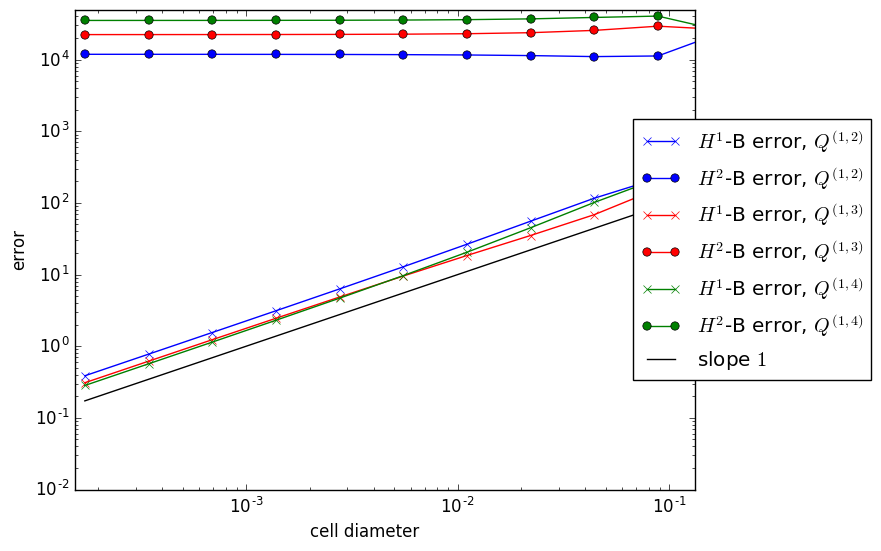
\includegraphics[width=3in]{Pictures/periodic-dont-eliminate-nonnormal-convergence.png}

        \caption{Convergence rates with anisotropic \(p\)-refinement. We do not
        recover any higher order accurate derivatives.}
    \end{figure}
\end{frame}

\begin{frame}
    \frametitle{Numerical Results}
    \begin{figure}
        \centering

        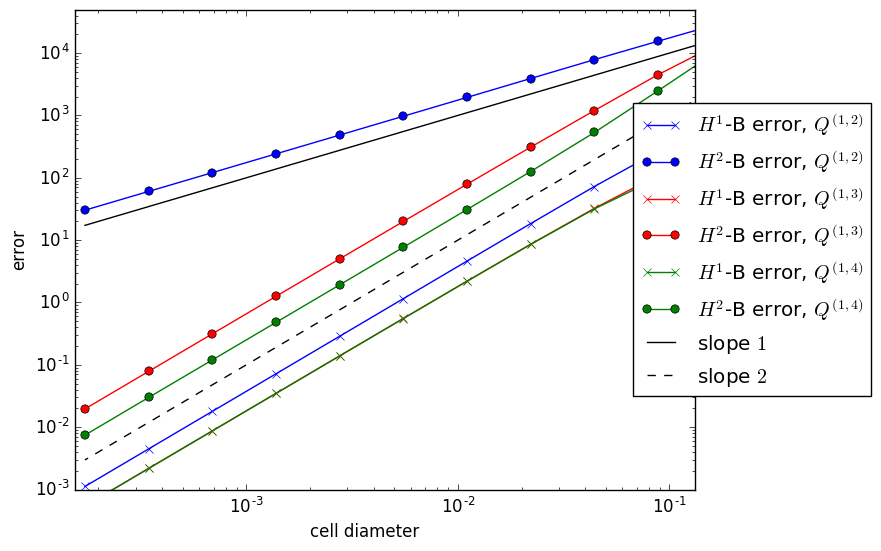
\includegraphics[width=3in]{Pictures/periodic-nonnormal-convergence.png}

        \caption{Convergence rates with isotropic \(p\)-refinement. The 1D
        theory applies at the knots.}
    \end{figure}
\end{frame}

\begin{frame}
    \frametitle{Numerical Results}
    \begin{figure}
        \centering

        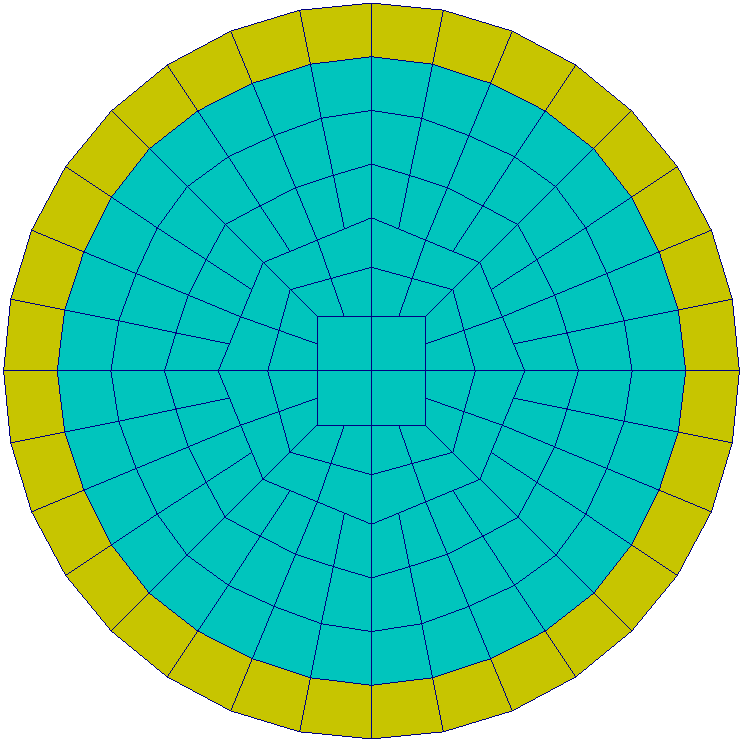
\includegraphics[width=2.5in]{Pictures/circular-grid.png}
        \caption{A circular grid with a geometry described near the boundary in
        polar coordinates, in the middle with Cartesian coordinates, and a
        transfinite interpolation in-between.}
    \end{figure}
\end{frame}

\begin{frame}
    \frametitle{Numerical Results}
    \begin{figure}
        \centering

        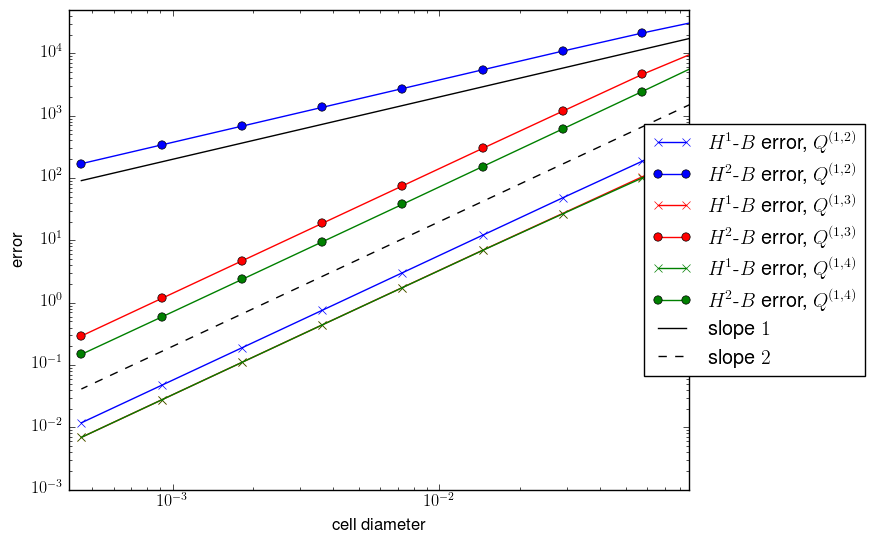
\includegraphics[width=3in]{Pictures/circle-nonnormal-convergence.png}
        \caption{Rates of convergence for the circular grid.}
    \end{figure}
\end{frame}

\section{Summary}
\begin{frame}
    \frametitle{Summary and Outlook}
    \begin{itemize}
        \item \(p\)-refinement error estimates involve a coupling term and a
              local term
        \item We can achieve higher-order derivative approximation at isolated
              points
        \item Future work: escape the Fourier framework, higher-order bulk
              elements, better tools for describing arbitrary geometries
    \end{itemize}
\end{frame}

\begin{frame}
    \begin{center}
    \textcolor{RPIred}{\Huge Thank You!}
    \end{center}
\end{frame}


\end{document}
